\documentclass{article}

\usepackage{booktabs}
\usepackage{tabularx}
\usepackage{hyperref}
\usepackage{graphicx}
\usepackage{pdflscape}

\def\fillandplacepagenumber{%
 \par\pagestyle{empty}%
 \vbox to 0pt{\vss}\vfill
 \vbox to 0pt{\baselineskip0pt
   \hbox to\linewidth{\hss}%
   \baselineskip\footskip
   \hbox to\linewidth{%
     \hfil\thepage\hfil}\vss}}
\hypersetup{
colorlinks=true,       % false: boxed links; true: colored links
linkcolor=red,          % color of internal links (change box color with linkbordercolor)
citecolor=green,        % color of links to bibliography
filecolor=magenta,      % color of file links
urlcolor=cyan           % color of external links
}

\title{Hazard Analysis\\\progname}

\author{\authname}

\date{}

%% Comments

\usepackage{color}

\newif\ifcomments\commentstrue %displays comments
%\newif\ifcomments\commentsfalse %so that comments do not display

\ifcomments
\newcommand{\authornote}[3]{\textcolor{#1}{[#3 ---#2]}}
\newcommand{\todo}[1]{\textcolor{red}{[TODO: #1]}}
\else
\newcommand{\authornote}[3]{}
\newcommand{\todo}[1]{}
\fi

\newcommand{\wss}[1]{\authornote{blue}{SS}{#1}} 
\newcommand{\plt}[1]{\authornote{magenta}{TPLT}{#1}} %For explanation of the template
\newcommand{\an}[1]{\authornote{cyan}{Author}{#1}}

%% Common Parts

\newcommand{\progname}{REVITALIZE} % PUT YOUR PROGRAM NAME HERE
\newcommand{\authname}{Team 13, REVITALIZE
\\ Bill Nguyen
\\ Syed Bokhari
\\ Hasan Kibria
\\ Youssef Dahab
\\ Logan Brown
\\ Mahmoud Anklis} % AUTHOR NAMES                  

\usepackage{hyperref}
    \hypersetup{colorlinks=true, linkcolor=blue, citecolor=blue, filecolor=blue,
                urlcolor=blue, unicode=false}
    \urlstyle{same}
                                


\begin{document}

\maketitle
\thispagestyle{empty}

~\newpage

\pagenumbering{roman}

\begin{table}[hp]
	\caption{Revision History} \label{TblRevisionHistory}
	\begin{tabularx}{\textwidth}{llX}
		\toprule
		\textbf{Date} & \textbf{Developer(s)} & \textbf{Change}\\
		\midrule
		October 15th, 2022 & Bill Nguyen & FMEA \\
		October 19th, 2022 & Youssef Dahab & Intro, Purpose, Scope, Roadmap \\
		October 19th, 2022 & Logan Brown & System Boundary, Components, and Critical Assumptions\\
		October 19th, 2022 & Syed Bokhari & FMEA\\
		October 19th, 2022 & Hasan Kibriai & FMEA\\
		October 19th, 2022 & Mahmoud Anklis & Safety and Security Requirements\\
		\bottomrule
	\end{tabularx}
\end{table}

~\newpage

\tableofcontents

\listoffigures


~\newpage

\pagenumbering{arabic}

\section{Introduction}
This document is a hazard analysis of REVITALIZE.

\subsection{Hazard Definition}
As per Nancy Leveson's work, a hazard is a property or condition in a system together with a condition in the environment that has the potential to cause harm or damage. In REVITALIZE, there are safety (keeping records) and security (restricting access to data) hazards.

\subsection{Other Used Terms in this Document}

\subsubsection{Failure}
A failure in the REVITALIZE mobile application could occur when there is a deviation between the actual and expected output. Furthermore, a failure could also occur when a certain state causes REVITALIZE, or a component of REVITALIZE (login, database, etc.), to fail and therefore not achieve its necessary function.

\subsubsection{Safety}
REVITALIZE's safety is its freedom from harm. However, it's not an absolute. Safety is a global property of REVITALIZE. Therefore, when two or more REVITALIZE components interact together, the resulting emergent behaviour may or may not be safe.

\section{Purpose of Hazard Analysis and Scope}
Hence, the purpose of this document is to identify hazards pertaining to the REVITALIZE mobile application, and their causes, and then specify ways to eliminate them or mitigate their effect. The team cannot “bolt on” safety after implementing the application. Therefore, by identifying hazards and developing safety requirements before implementing, REVITALIZE team members will be able to react when their application fails to be safe. This becomes beneficial when something “bad” happens. The team will have a recovery plan.
\\\\ The scope of this project is to create an all in one health and wellness mobile application that allows users to manage their diet, exercise, and sleep by providing them with meal recipe’s based on their nutritional preferences, a personalized workouts planner and a sleep tracker.

\section{System Boundaries and Components}

\subsection{System Boundaries}
\noindent The system boundary can be outlined using the following elements of the system: 

\begin{enumerate}
	\item Main application (with the following subsystems)
	\begin{itemize}
		\item Login/Authentication
		\item Database
		\item Backend server
		\item Main calendar
		\item Diet menu
		\item Workout menu
		\item Sleep menu
	\end{itemize}
	\item APIs
	\begin{itemize}
		\item Recipe API
		\item Workout tracker API
		\item Google sleep tracker API
	\end{itemize}
	\item Android device (device app is installed on)
\end{enumerate}

\noindent The system boundary includes the application as a whole, the APIs used for its function, and the Android device the app is installed onto. Some of these elements are outside the direct control of REVITALIZE, namely the APIs, server uptime, database uptime, and the Android device itself. However, they are important elements of the system that must be taken into account for proper hazard analysis of the system.

\subsection{Components}

\noindent The components of the system are outlined as followed:

\subsubsection{Login/Authentication System}
\noindent System that allows users to create an account, login, and have their credentials verified. Users can then access their data and modify health goals and plans.

\subsubsection{Database}
\noindent System that stores and organizes user health data. Data will be stored to the user's account and is accessible to any device that logs in with said account.

\subsubsection{Server Backend}
\noindent System that controls the flow of data between the APIs and the application.

\subsubsection{Main Calendar Interface}
\noindent System that displays current diet, workout, and sleep goals/plans for selected day. Users can select a desired day on the calendar and navigate to the diet, workout, and sleep interfaces which are used to modify user goals and plans.

\subsubsection{Diet Section Interface}
\noindent System that allows users to search and add recipes aligned with their dietary goals. The recipes chosen by the user are then added to the plan of the selected day. Previously planned recipes are stored for easy access in the future.

\subsubsection{Workout Section Interface}
\noindent System that allows users to add existing or custom workouts to the selected calendar day. Previous workouts are stored for easy access in the future. 

\subsubsection{Sleep Section Interface}
\noindent System that tracks and displays user sleep data. Also displays sleep/wake-up times based on user sleep goals and habits. 

\section{Critical Assumptions}
\noindent 
\begin{enumerate}
	\item Assume user is not intentionally acting in a malicious way
	\item Assume user is not sharing username and password info with anyone else
	\item Assume user's Android device is functioning properly
	\item Assume user's Android device does not contain any vulnerabilities
	\item Assume APIs are up and function properly
	\item Assume APIs do not contain any vulnerabilities
\end{enumerate}

\section{Failure Mode and Effect Analysis}
The next pages will show the full failure mode and effect analysis (FMEA) for REVITALIZE:
\begin{landscape}
	\begin{figure}[ht]
		\centering
		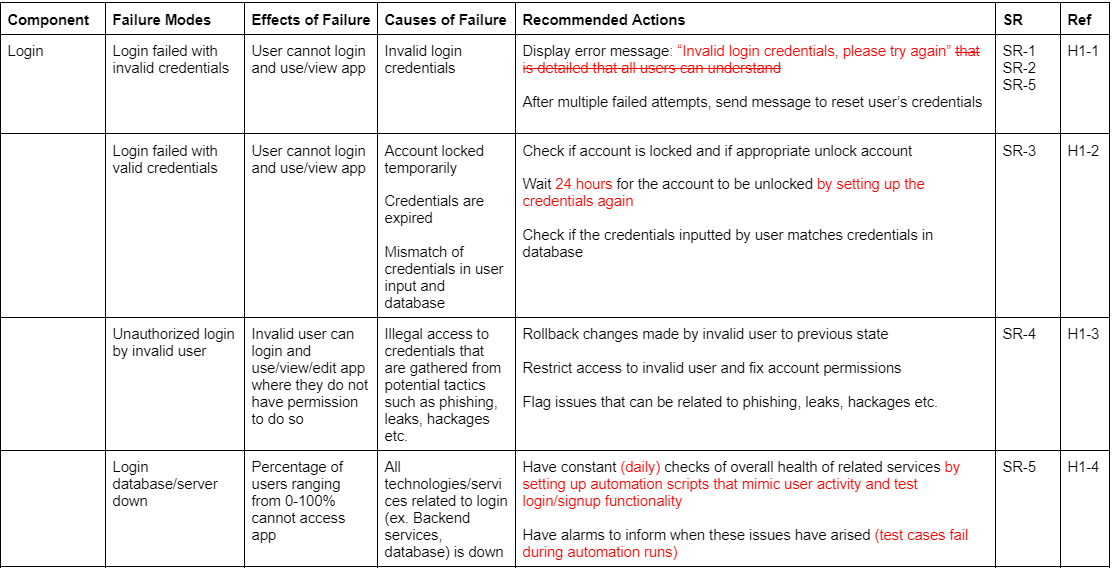
\includegraphics[angle=360, scale=0.8]{FMEA_1.png}
		\caption{Part 1 of FMEA}
	\end{figure}
	\fillandplacepagenumber
\end{landscape}
\begin{landscape}
	\begin{figure}[ht]
		\centering
		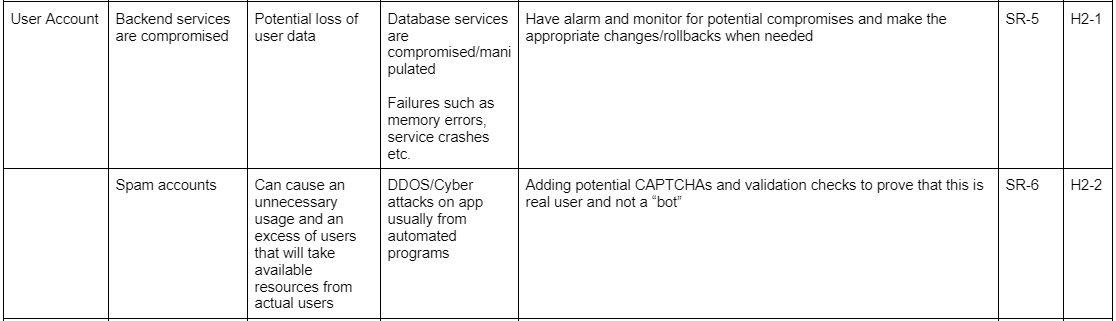
\includegraphics[angle=360, scale=1.15]{FMEA_2.png}
		\caption{Part 2 of FMEA}
	\end{figure}
	\fillandplacepagenumber
\end{landscape}
\begin{landscape}
	\begin{figure}[ht]
		\centering
		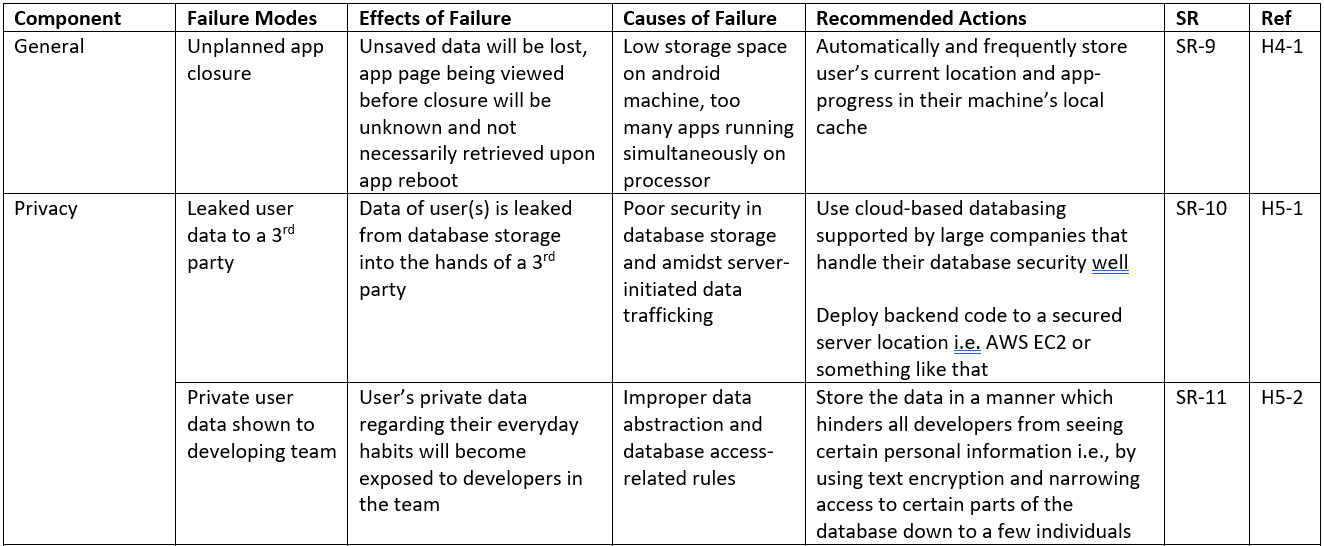
\includegraphics[angle=360, scale=0.85]{FMEA_3.png}
		\caption{Part 3 of FMEA}
	\end{figure}
	\fillandplacepagenumber
\end{landscape}

\begin{landscape}
	\begin{figure}[ht]
		\centering
		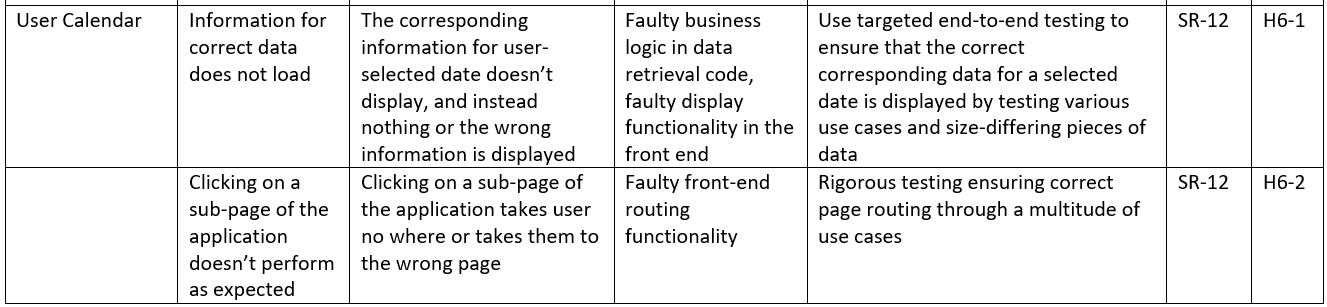
\includegraphics[angle=360, scale=1]{FMEA_4.png}
		\caption{Part 4 of FMEA}
	\end{figure}
	\fillandplacepagenumber
\end{landscape}

\begin{landscape}
	\begin{figure}[ht]
		\centering
		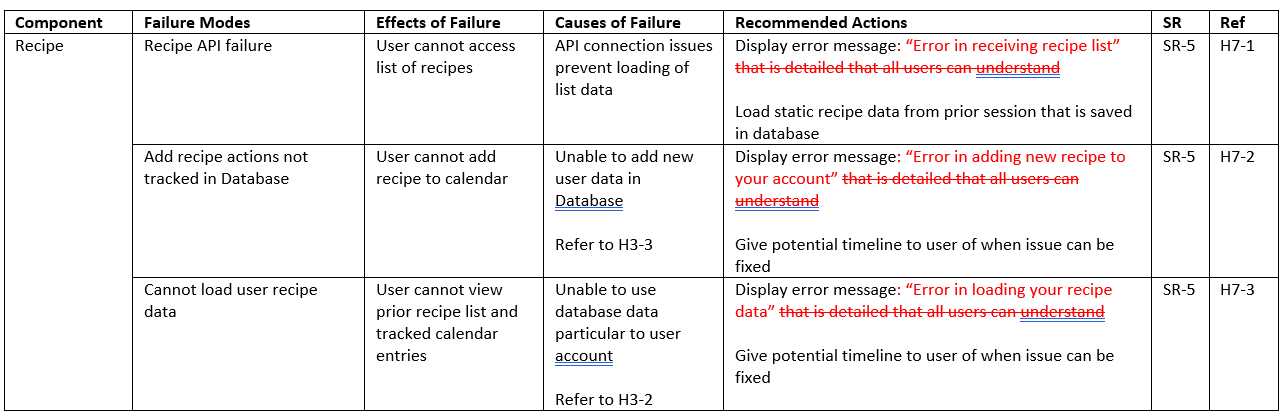
\includegraphics[angle=360, scale=1]{FMEA_5.png}
		\caption{Part 5 of FMEA}
	\end{figure}
	\fillandplacepagenumber
\end{landscape}

\begin{landscape}
	\begin{figure}[ht]
		\centering
		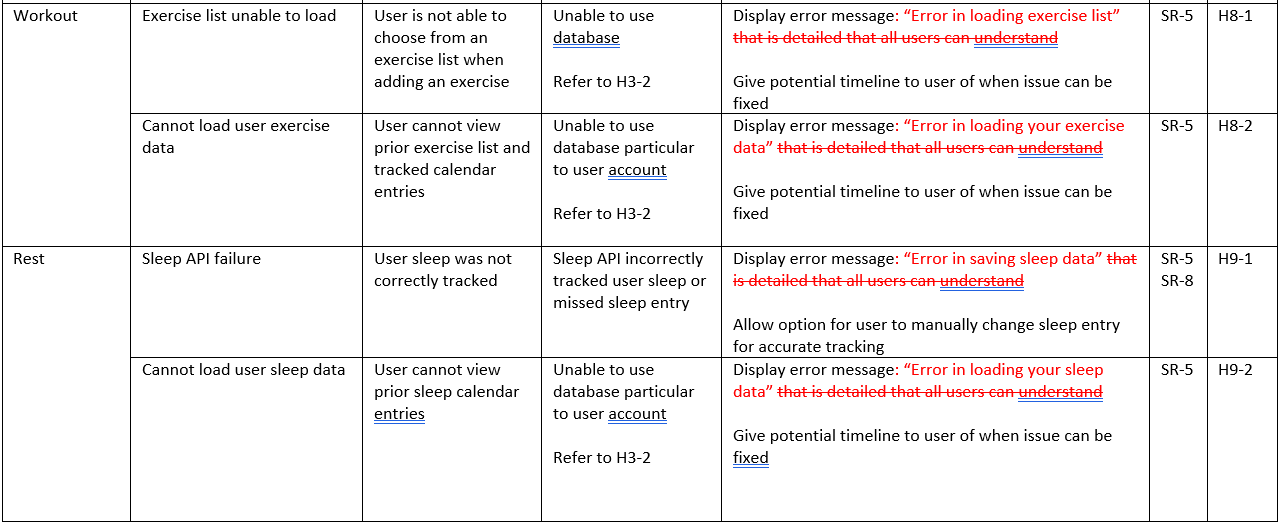
\includegraphics[angle=360, scale=0.9]{FMEA_6.png}
		\caption{Part 6 of FMEA}
	\end{figure}
	\fillandplacepagenumber
\end{landscape}

\section{Safety and Security Requirements}
\begin{enumerate}
	\item The system should check if the credentials inputted by the user match the credentials in the database.
	\begin{enumerate}
		\item Rationale: The user should be able to access their account if the credentials are inputted correctly (i.e matches the database).
		\item Associated Hazards
		\begin{enumerate}
			\item H1-1
		\end{enumerate}
	\end{enumerate}
	\item The system should allow users to reset credentials if a user requests it.
	\begin{enumerate}
		\item Rationale: In the case that a user forgets their password or username, they should be able to retrieve their account be resetting the credentials.
		\item Associated Hazards
		\begin{enumerate}
			\item H1-1
		\end{enumerate}
	\end{enumerate}
	\item The system should lock a user’s account when the user has inputted the incorrect password 5 times in a row.
	\begin{enumerate}
		\item Rationale: To ensure that the account is secured, the account of a user will get locked if multiple unsuccessful login attempts occur. 
		\item Associated Hazards
		\begin{enumerate}
			\item H1-2
		\end{enumerate}
	\end{enumerate} 
	\item The system should be able to roll back changes. 
	\begin{enumerate}
		\item Rationale: To ensure the user does not lose their data if an illegal access or a system failure occur and can continue using the application.
		\item Associated Hazards
		\begin{enumerate}
			\item H1-3, H3-1
		\end{enumerate}
	\end{enumerate} 
	\item The system notifies users when the system is down (planned outings or unexpected outings) or when an error occurs and when the system will be back online. 
	\begin{enumerate}
		\item Rationale: Users can avoid using the application or parts of the application during these times. 
		\item Associated Hazards
		\begin{enumerate}
			\item H1-1, H1-4, H2-1, H3-2, H3-3, H7-1, H7-2, H7-3, H8-1, H8-2, H9-1, H9-2
		\end{enumerate}
	\end{enumerate}
	\item The system should limit the number of bots using the application.
	\begin{enumerate}
		\item Rationale: The application is intended for human users.
		\item Associated Hazards
		\begin{enumerate}
			\item H2-2
		\end{enumerate}
	\end{enumerate}
	\item The system will have daily backups to multiple databases.
	\begin{enumerate}
		\item Rationale: Redundancy in data will ensure the safety of the data and protect it from being lost.
		\item Associated Hazards
		\begin{enumerate}
			\item H3-1
		\end{enumerate}
	\end{enumerate}
	\item The system allows the user to manually input sleep information.
	\begin{enumerate}
		\item Rationale: The sleep functionality can still be used in the case of a sleep API failure.
		\item Associated Hazards
		\begin{enumerate}
			\item H9-1
		\end{enumerate}
	\end{enumerate}
	\item The system should store app-progress information on the user’s local machine.
	\begin{enumerate}
		\item Rationale: Easier and quicker to access information if stored in machine’s local cache.
		\item Associated Hazards
		\begin{enumerate}
			\item H4-1
		\end{enumerate}
	\end{enumerate}
	\item The system should use cloud-based databases.
	\begin{enumerate}
		\item Rationale: Provides greater security to users’ data.
		\item Associated Hazards
		\begin{enumerate}
			\item H5-1
		\end{enumerate}
	\end{enumerate}
	\item The system will use encryption when storing users’ information.
	\begin{enumerate}
		\item Rationale: Provides security for users’ data and ensures developers cannot see users’ data.
		\item Associated Hazards
		\begin{enumerate}
			\item H5-2
		\end{enumerate}
	\end{enumerate} 
	\item The system will incorporate rigorous weekly testing.
	\begin{enumerate}
		\item Rationale: Ensures proper functionality.
		\item Associated Hazards
		\begin{enumerate}
			\item H6-1, H6-2
		\end{enumerate}
	\end{enumerate} 
\end{enumerate}

\section{Roadmap}
The REVITALIZE team's hazard mitigation strategy began first with identifying potential hazards and then creating new safety and security requirements to mitigate those hazards. This has been accomplished in the previous two sections. After that, each hazard was mapped to its corresponding safety or security requirement. Many of the listed hazards have a medium or high chance of occurring. Hence, SR-1 to SR-5, SR-8, and SR-10 to SR-12 will be implemented as part of the capstone timeline. H2-2, H3-1 and H4-1 have a lower probability of occurring. Therefore, SR-6, SR-7 and SR-9 will be implemented in the future. The last steps in the REVITALIZE team's hazard mitigation strategy entail developing the application and testing to verify that safety and security requirements have been met. If they have, then the hazards corresponding to that particular safety or security requirement have been successfully mitigated. The team is aware that future potential vulnerabilities could arise where they will have to be assessed based on severity and probability of occurrence.

\end{document}